\chapter{Discussion}

The topics covered by this chapter will be about :

\begin{description}
	\item[Nfsen] We began our master thesis by trying to implement a plug in for that particular software. Details will be given on how this tool work and reasons will be given on why we abandoned the idea of of implementing a plug in. However, as you will see, our architecture resembles a lot to Nfsen.
	\item[Possible extensions] Those are features that could be added to our current software as to improve it.
	\item[Security] Issues about security will be addressed.
\end{description}

\section{Nfsen, A Graphical Web Tool}

\begin{figure}[!h]
	\centering
	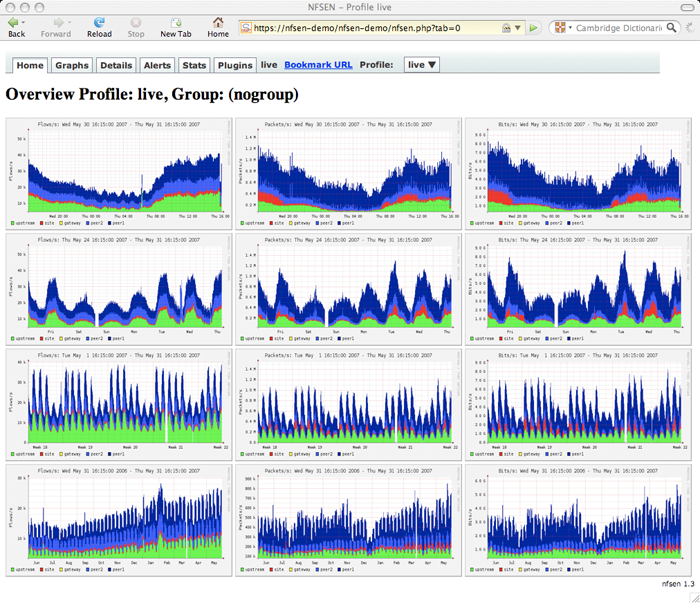
\includegraphics[width=0.8\textwidth]{res/nfsen.png}
	\caption{The Nfsen interface (source : \url{nfsen.sourceforge.net})}
	\label{fig:nfsen}
\end{figure}

The subject of our master thesis having been proposed by Professor Sadre last year and being about monitoring flows in IoT networks, the first tool that was presenting itself to us was Nfsen. Per its official website, \textit{Nfsen is a graphical web based front end for the nfdump netflow tools}. The Nfsen tool uses various graphes and charts to display the traffic of data varying with a specified time span or time interval. It works with the processing capabilities of Nfdump, a data processing tool using Netflow flows that have been retrieved from a network. Specifically, the Nfsen interface also allows to create plugins to have more ways of displaying data information. At first, it was proposed in the description of the subject of the thesis to use Nfsen along with Nfdump, particularly creating an Nfsen addon to show further information along with what Nfsen already is displaying in terms of graphical content. By plugin, one graphical content that Nfsen is lacking is the current topology of the monitored network, which can be added by making a plugin which extends the graphical tool.\\

In this section, we will explain all the underlying layers of Nfsen, from data exchanged in the monitored network to the graphical web page. We will also discuss our thought process about using Nfsen and the reasons why we have not used it in the end.\\

The first step towards monitoring is data collecting. As we explained in Chapter 3, Netflow is used for collecting flows we are interested in, according to some specific attributes such as the source and destination addresses. Once the flow are captured, they are stored and waiting to be processed. \\

In reality, when the structure of the Netflow data is defined, the flows are actually captured by \textit{nfcapd}, a \textit{netflow capture deamon}. With nfcapd, the flows are read from the network and the collected data is stored into files, data being split in files according to time slices. Each five minutes, nfcapd outputs a new file where data is stored, named with the current timestamp. One nfcapd process is used for each existing netflow stream that we want to capture.\\

As seen in the next figure, the next important component is \textit{nfdump}. Nfdump is a command line based tool that provides further data processing. Basically, it reads the data that was previously captured and stored by nfcapd. With Nfdump, data is aggregated and it provides further statistics about the traffic. Nfdump can either analyze the data coming from a single file, or from several of them by concatenating them before analyzing. One strength of nfdump is that it can filter out the attributes in the data that are not needed during the processing. Afterwards, the data is output either as a text file or binary data, thus being ready for further analysis. Nfdump aggregates and then creates statistics about the flows information stored, such as traffic volume sent during a timelapse. Nfdump thus acts as the backend of Nfsen.\\

\begin{figure}[!h]
	\centering
	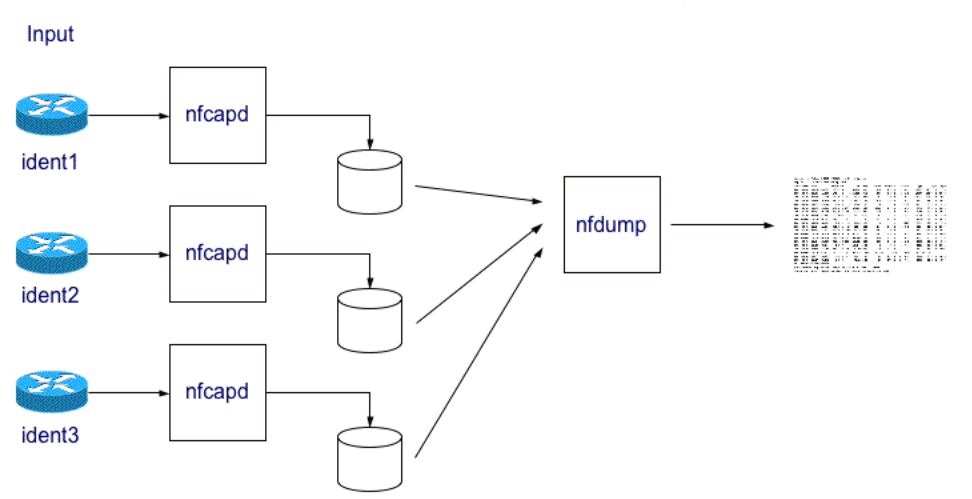
\includegraphics[width=0.8\textwidth]{res/nfdump.png}
	\caption{The Nfdump Structure (source : \url{nfdump.sourceforge.net})}
	\label{fig:nfdump}
\end{figure}

Once the data is processed, it is displayed by Nfsen with the help of graphs. Nfsen displays the collected netflow data, either in flows, packets, or bytes. As you can see in figure \ref{fig:nfsen}, it can display various types of data, for example data sent through different protocols such as UDP, TCP, etc. It also uses time spans to select which data traffic is to be displayed (being the same time spans where nfdump did all the processing).\\

As stated earlier, Nfsen can also be extended, by creating plugins. There exist two kinds of plugins. There are the backend plugins that are written in Perl, that are created to add more functions and functionalities such as alerting conditions and data processing. On the other hand, frontend plugins are written in PHP and used to create new display fashions that the original Nfsen application would lack. In our case, we wanted to display the topology of the network under analysis, which Nfsen is not showing in its original state. Note that each backend plugin should be associated with its respective frontend plugin.

\subsection{Nfsen \& Nfdump, not best suited?}

In section 5.1, we talked about Nfsen and how it is possible to create plugins to have further monitoring capabilities. As stated, the first description of the thesis was to create an \textit{Nfsen plugin} to visualize an IoT network in an Ad Hoc manner, with devices having Netflow activated.\\

At the beginning of this school year, once we started working on our thesis, we dug into Nfsen and its functionalities, trying to get familiar with it. First of all, setting up the Nfsen tool showed itself to be very tedious and challenging, as many installation tutorials did not work for all computers and OSs, and had different instructions.\\

The main reason why Nfsen is useful is that it easily and immediately treats the netflow information retrieved by nfcapd and nfdump, with little to no addition and/or modification needed. However, as we had decided to design our own IPFIX fields to visualize IoT networks according to our needs, we also had to modify nfdump. Namely, two fields that the original IPFIX structure does not monitor, and hence are not standardized fields, are the battery level of devices and the parent of each mote in the IoT networks. Digging into nfdump seems to require quite some time and some knowledge of the Perl language. Entering the last year of our master thesis, we also had never used nor learned the PHP and perl languages in contrary to Javascript with the Node.js framework. \\

Thinking of using the Node.js framework seemed reasonably more practical in our case in terms of time allocation, since we required to modify the netflow information retrieved from networks. With further discussion, we decided to write a Javascript program that played the role of Nfdump to efficiently parse and store the netflow information captured. Similarly, instead of using nfsen as the graphical interface, we programmed a web tool with Node.js to be able to visualize information in which we are interested in. Of course, our graphical interface is less complete than nfsen's, but it contains a topology showcase that nfsen does not, that we have programmed using the D3.js library as explained earlier.\\

In the end, Nfsen used with Nfdump present a lot of advantages, as most of the work is already present in its core, only a few things have to be added, i.e. the topology here. It contains a lot of graphical information on how much traffic passes through the network, with many filters such as graphs split according to which protocols send the information. But for the reasons we have cited above, we have decided not to use it and opted for a solution using Node.js.

\section{Possible Extensions}

\subsection{Load of data on Links}

In this master thesis, we have mostly focused on data creation from nodes and passing through nodes, since Netflow is activated on the said nodes. We have not implemented features allowing to monitor traffic passing through specific links, as it would require a few modifications in the way we process data, and would also add more traffic load in the IoT network.\\

In the situation where we would have implemented monitoring mechanisms for data passing through links, we could have used the topology and an opacity chart to show where loads of data are mostly generated from and flowing through, as you can see in figure \ref{fig:opacity}. Using tresholds for bytes of data passing through links, we would use a darker opacity for huge loads of data, and a lighter opacity if not much data passes through a certain link.

\begin{figure}[!h]
	\centering
	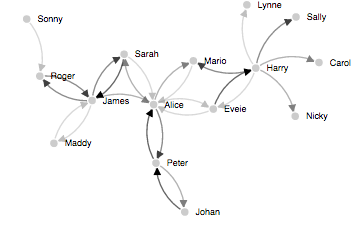
\includegraphics[width=0.8\textwidth]{res/opacity.png}
	\caption{Opacity on links (source : \url{http://bl.ocks.org/d3noob/5155181})}
	\label{fig:nfsen}
\end{figure}

\subsection{Topology according to real position}

As of now, the topology feature showcases a network toplogy that only depends on which motes are communicating to each other, no matter what is the relative position of those motes according to others in the network. \\

A possible extension could be to showcase a topology where its nodes are positioned as in real life, with a corresponding proportional distance. However, that would imply adding complexity on each mote to have a feature computing the distances and angles formed from each three nodes, and that would also induct a raise in traffic volume since more packets containing position information are to be exchanged.

\subsection{Network failure}

When developing the software, we have not made any assumption that links and nodes may potentially fail. As of now, the way the topology updates itself is by refreshing the page and thus showcasing the topology. The topology is built according to netflow packets that are sent from the network to the server, which is everytime the server receives a flow of netflow packets. In reality, a topology change may come from a link failure, i.e. two nodes may have difficulties communicating together, or node failures if a mote runs out of battery or is accidently broken. \\

One important aspect to take into account is the fact that the topology is organized as a tree, meaning for each node or link failing, there is a cascade of nodes down branches that will consequently not be able to communicate with the gateway node. Of course, the gateway node is a \textit{Single Point of Failure} (see figure \ref{fig:spof}), since it failing would completely cut the communication between the IoT network and the server, thus not having any information on the network anymore.\\

\begin{figure}[!h]
	\centering
	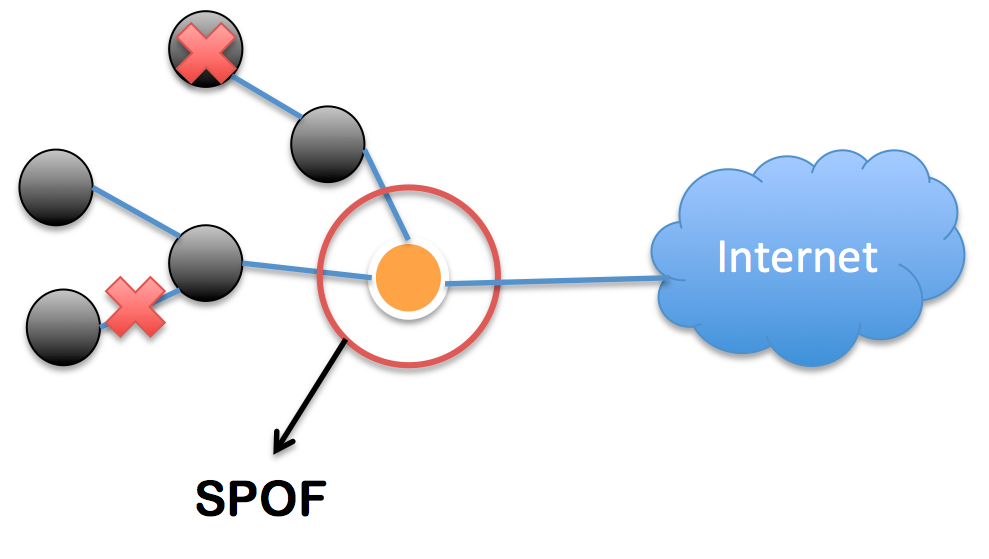
\includegraphics[width=0.8\textwidth]{res/spof.png}
	\caption{Tree topology, link and node failure, SPOF}
	\label{fig:spof}
\end{figure}

A potential extension could be to have a panel showcasing the \textit{previous topology} after an update of topology, allowing to make comparisons between the current and the previous network state, and thus see if there potentially was an important change in the network.\\

As stated, the topology is updated according to netflow packets and information retrieval. In the network's current state, a mote that has not sent information for a while or a mote that has failed and that has consequently not sent any information would be interpeted the same way in our topology. \\

Further mechanisms are needed to be able to distinguish the two situations, such as adding some field in our TinyIPFIX structure in combination with \textit{Hello packet} exchanges between a parent node and its childs to test reachability. Plus, it allows to have some information on downstream nodes and send that information to the gateway node. Those solutions require more lines of code on each mote, and a modified netflow structure with added fields.



\subsection{Protocols distribution}

As of now, our software does not have the possibility to sort the flows by protocols (RPL, UDP, TCP, ...). An improvement of our solution could permit to differentiate flows depending on the protocols. However, to effectively enable such feature, the records sent by the nodes should contain more data. This implies that the nodes would send more data and a study of the impact on the nodes battery life would be necessary.

\section{Security}

Throughout the thesis, security has not been the main point of focus. Indeed, we have not implemented any security mechanism, inside the IoT network nor between the gateway node and our server. Data not being encrypted may be an issue as the communication between devices in the network becomes a target for sniffing and packets tempering. Of course, one direct impact of such insecurity is that data to be processed that is sent to the server may be tempered and thus, later on, the monitoring software would showcase wrong information about the traffic load and the topology for example.\\

Purely from a theoretical point of view, there is also a lack of security between devices inside the network, but also between the gateway mote and the server, communicating via UDP. The sniffing of exchanged packets can be an issue, as well as identity theft (spoofing) where a third party could act as, for instance, being the gateway mote and send data to the server, because of the lack of authentication when communication is opened. \\

Authentication mechanisms and encryption are the way to go to solve these problems. We would thus have authentication between motes (only gateway mote and server?), and encryption of data when creating packets from motes. However, those mechanisms add lines of codes uploaded on motes, which must be taken into account when analyzing and optimizing performances of the IoT network. In consequence, the mechanisms also add more traffic load to the network.\\

All those points are to be taken into account to showcase accurate data. In our case though, no tempering was possible, as we knew exactly what kind of data passes through the network and which device creates the flows.
